\begin{filecontents}{ref.bib}
@article{GELADE20102987,
	title = "Succinctness of regular expressions with interleaving, intersection and counting",
	journal = "Theoretical Computer Science",
	volume = "411",
	number = "31",
	pages = "2987 - 2998",
	year = "2010",
	note = "",
	issn = "0304-3975",
	doi = "http://dx.doi.org/10.1016/j.tcs.2010.04.036",
	url = "http://www.sciencedirect.com/science/article/pii/S0304397510002537",
	author = "Wouter Gelade",
	keywords = "Regular Expressions",
	keywords = "Succinctness"
}
\end{filecontents}

\documentclass{article}

\usepackage[margin=3cm]{geometry}
\usepackage{amsmath}
\usepackage{amssymb}
\usepackage[noend]{algorithm2e}
\usepackage{xspace}
\usepackage{enumerate}
\usepackage{tikz}
\usetikzlibrary{positioning, automata}
\usepackage{caption}
\usepackage{subcaption}
\usepackage{float}

\title{\Large\bfseries CS 598: Runtime Verification \\
Spring 2017 \\
Homework 2}
\author{Chiao Hsieh, chsieh16@illinois.edu}

\begin{document}
\maketitle

\newcommand{\FinTraces}{\ensuremath{\Sigma^*}\xspace}
\newcommand{\InfTraces}{\ensuremath{\Sigma^\omega}\xspace}
\newcommand{\prefixes}{\ensuremath{\mathtt{prefixes}}\xspace}
\newcommand{\Nat}{\ensuremath{\mathbb{N}}\xspace}
\newcommand{\Real}{\ensuremath{\mathbb{R}}\xspace}
\newcommand{\Bool}{\ensuremath{\mathbb{B}}\xspace}

\newcommand{\Lang}{\ensuremath{\mathcal{L}}}


\begin{enumerate}
\item Give pseudo-code for the problem of generating a minimal BTT for a given
MT (described in Section 6.1.2 and right after Definition 36)

Ans.

Let the set of multi-transitions $MT(P_A, S)$ over the set of states $S$ and
propositions $P_A$ over atom predicates $A$,
Algorithm~\ref{alg:mt2btt} generates minimal BTT for a given nondeterministic MT.

\newcommand{\TT}{\ensuremath{{a=1}}}
\newcommand{\FF}{\ensuremath{{a=0}}}

\begin{algorithm}

\KwIn{$mt = [p_1:s_1, p_2:s_2, \dots, p_n:s_n] \in MT(P_A, S)$}
\KwOut{$b \in BTT(A, S)$}
\BlankLine

\SetKwProg{KwFn}{function}{}{end}

\SetKwFunction{MinBTT}{MT2MinBTT}
\SetKwFunction{min}{min\_cost}s
\KwFn{\MinBTT{mt, A}}{
	$b = \epsilon$\;
	\If{$A = \emptyset$}{
		\ForEach{$p_i:s_i \in mt$}{
			\If{$p_i$ is valid}{
				$b$ = $b\ s_i$\;
			}
		}
	}
	\Else{
		\ForEach{$a \in A$}{
			$mt^\TT = [p_1^\TT:s_1, p_2^\TT:s_2, \dots, p_n^\TT:s_n]$\;
			$b^\TT$ = \MinBTT{$mt^\TT$, $A\setminus\{a\}$}\;
			$mt^\FF = [p_1^\FF:s_1, p_2^\FF:s_2, \dots, p_n^\FF:s_n]$\;
			$b^\FF$ = \MinBTT{$mt^\FF$, $A\setminus\{a\}$}\;
			$b^a = a? b^\TT: b^\FF$\;
			$b$ = \min{b, $b^a$}\;
		}
	}
	\KwRet $b$\;
}
\caption{MT to BTT Algorithm}\label{alg:mt2btt}

\end{algorithm}

In particular, $p_i^{a=v}$ means simplifying proposition $p_i$ by replacing all
occurrence of atomic predicate $a$  with value $v$.
Cost of a given BTT can be calculated based on Section 6.2.

\item Does the lower bound result in Section 7.1 hold for semi-extended regular
expressions, that is, for regular expressions extended only with intersection
($\cap$) but not negation ($\neg$)? If yes, then sketch a proof. If no, then
explain why not and try to find another lower bound.

Ans.

No, the lower bound result does not apply to semi-extended regular
expressions~(SERE).
A simple explanation is that there is an algorithm in~\cite{GELADE20102987} to
construct an NFA from a given SERE, $r$,  that the size of the NFA is with at most
$2^{|r|}$ states.

A lower bound is proven by Theorem 8 in~\cite{GELADE20102987} that there can be
a SERE, $r$, with $n$ intersection operators such that any DFA accepting
$\Lang(r)$ contains at least $2^{2^n}$ states.


\item Implement the derivative-based ERE membership checking algorithm described
in Section 7.2.2 (see also Theorem 10). Use your favorite programming language.

Ans.

\newcommand{\G}{\ensuremath{\square}}
\newcommand{\F}{\ensuremath{\diamond}}
\newcommand{\U}{\ensuremath{\ \mathcal{U}\ }}

\item As seen in Chapters 8 and 9, there are different semantics for LTL.
This can be quite confusing in practice, because one can write a safety property
using LTL thinking of one semantics, say finite-trace semantics, but then use
the monitor generation algorithm for the other semantics, say infinite-trace.
(1) Give an LTL formula which is valid under one semantics but not under the other.
(2) Give an LTL formula whose languages of bad-prefixes are different under the
    two semantics.
(3) Describe an implementation that automatically checks whether a given formula
    admits different bad prefixes under finite-trace vs. infinite-trace semantics.

Ans.

\begin{enumerate}[(1)]
\item Given LTL formula $\varphi = \F (\G p \lor \G \neg p)$, the formula is valid in the
finite-trace semantic defined in Section 8.1.1 but not valid in infinite-trace
semantic.
The reason is because, for any given trace $t$, we can always find the suffix
trace $t_i$ with $i = Length(t)$, so $t_i$ contains only one event $e = head(t_i)$
and $Length(t_i) = 1$.
Since it's either $p \in e$ or $p \notin e$,we know that
$(\forall j \leq 1) t_{ij} \models p$ or $(\forall j \leq 1) t_{ij} \models \neg p$
where $t_{ij} = e$ is the only suffix of $t_i$.
Therefore, the formula always holds.

However, this is not valid for infinite trace semantic.
A counter-example infinite trace is $(ab)^\omega$ over $\Sigma =\{a,b\}$,
and the atomic predicate is $a$.
We can never find a suffix such that $a$ always holds or never holds.

\item Consider the negation of the formula in (1), since $\varphi$ is valid
for finite-trace semantic,
we know $\neg \varphi$ is unsatisfiable, i.e., $\Lang(\neg\varphi) = \emptyset$.
A bad-prefix of $\Lang(\neg\varphi)$ is therefore any trace in $\Sigma^*$.

However, if we consider infinite-trace semantic,
the bad-prefixes for $\Lang(\neg\varphi)$ is clearly not $\Sigma^*$.

\item 

\textcolor{red}{
Given $\varphi$, try to construct $ \varphi \land \psi$ so that
$\psi$ describes the stutter when finite trace is extended to infinite trace.
And then maybe check the validity of $\varphi \leftrightarrow \varphi \land \psi$
}

\end{enumerate}


\item Consider the following three (infinite-trace) LTL formulae from Table 9.2:
$\G(a\land b \to \F c)$, $\G(a \to b \U c)$, and,
respectively, $a\land\circ(\F b)\land \F(\G(e))$
For each of them do the following:
(1) give a Buchi automaton that has the same language;
(2) give an MFSM corresponding to (1) that rejects precisely the minimal bad
prefixes (see Theorem 18);
(3) optimize the MFSM in (2) by collapsing the non-monitorable states (algorithm
in Figure 9.4);
(4) give the optimal BTT-FSM corresponding to (3).

Ans.

\renewcommand{\thesubfigure}{\arabic{subfigure}}
\tikzset{
	->, node distance=2cm,
	every loop/.style={min distance=10mm,in=70,out=110}
}
\begin{figure}[H]
	\centering
	\caption{$\square(a\land b \to \diamond c)$}
\begin{subfigure}[t]{0.35\textwidth}
	\centering
	\caption{B\"uchi Automaton}
	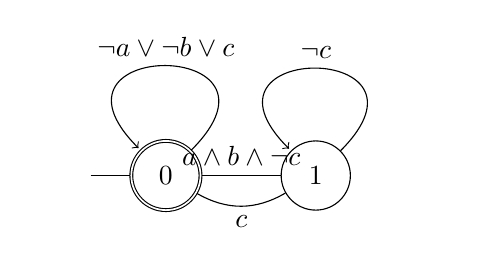
\begin{tikzpicture}	
	\node (init) {};
	\node [state, accepting, right=0.5cm of init](0) {0};
	\node [state, right=of 0] (1) {1};
	
	\path
		(init) edge (0) 
		(0) edge [loop] node[above]{$\neg a\lor\neg b \lor c$} (0)
		(0) edge node [above] {$a \land b \land \neg c$} (1)
		(1) edge [loop] node [above] {$\neg c$} (1)
		(1) edge [bend left] node [below] {$c$} (0)
	;
	\end{tikzpicture}
\end{subfigure}
\begin{subfigure}[t]{0.35\textwidth}
	\centering
	\caption{MFSM}
	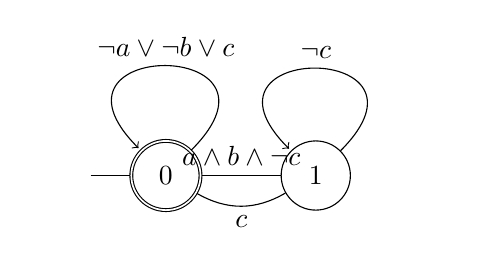
\begin{tikzpicture}
	\node (init) {};
	\node [state, accepting, right=0.5cm of init](0) {0};
	\node [state, right=of 0] (1) {1};

	\path
		(init) edge (0) 
		(0) edge [loop] node[above]{$\neg a\lor\neg b \lor c$} (0)
		(0) edge node [above] {$a \land b \land \neg c$} (1)
		(1) edge [loop] node [above] {$\neg c$} (1)
		(1) edge [bend left] node [below] {$c$} (0)
	;
	\end{tikzpicture}
\end{subfigure}
\begin{subfigure}[t]{0.2\textwidth}
	\caption{Collapsing}
	\centering
	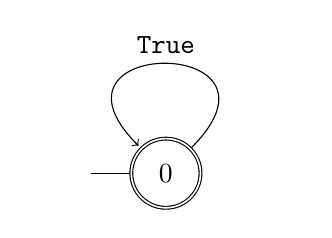
\begin{tikzpicture}
	\node (init) {};
	\node [state, accepting, right=0.5cm of init](0) {0};
	
	\path
		(init) edge (0) 
		(0) edge [loop] node[above]{\texttt{True}} (0)
	;
	\end{tikzpicture}
\end{subfigure}

\begin{subfigure}[t]{0.4\textwidth}
	\caption{BTT-FSM}
	\centering
	$[neverViolate] \rightsquigarrow neverViolate$
\end{subfigure}
\end{figure}

\begin{figure}[H]
	\centering
	\caption{$\G(a \to b \U c)$}
\begin{subfigure}[t]{0.3\textwidth}
	\caption{B\"uchi Automaton}
	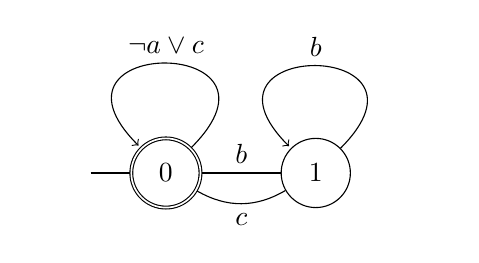
\begin{tikzpicture}	
	\node (init) {};
	\node [state, accepting, right=0.5cm of init](0) {0};
	\node [state, right=of 0] (1) {1};
	
	\path
		(init) edge (0) 
		(0) edge [loop] node[above]{$\neg a\lor c$} (0)
		(0) edge node [above] {$b$} (1)
		(1) edge [loop] node [above] {$b$} (1)
		(1) edge [bend left] node [below] {$c$} (0)
	;
	\end{tikzpicture}
\end{subfigure}
\begin{subfigure}[t]{0.3\textwidth}
	\caption{MFSM}
	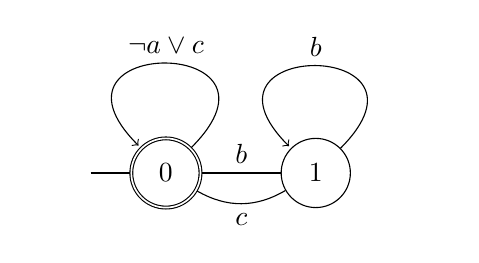
\begin{tikzpicture}	
	\node (init) {};
	\node [state, accepting, right=0.5cm of init](0) {0};
	\node [state, right=of 0] (1) {1};
	
	\path
	(init) edge (0) 
	(0) edge [loop] node[above]{$\neg a\lor c$} (0)
	(0) edge node [above] {$b$} (1)
	(1) edge [loop] node [above] {$b$} (1)
	(1) edge [bend left] node [below] {$c$} (0)
	;
	\end{tikzpicture}
\end{subfigure}
\begin{subfigure}[t]{0.3\textwidth}
	\caption{Collapsing}
	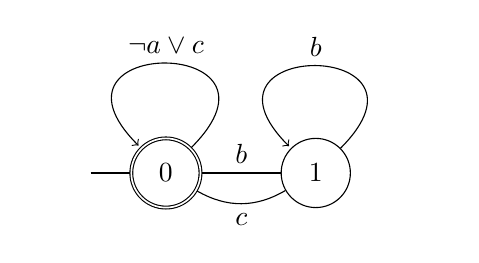
\begin{tikzpicture}	
	\node (init) {};
	\node [state, accepting, right=0.5cm of init](0) {0};
	\node [state, right=of 0] (1) {1};
	
	\path
	(init) edge (0) 
	(0) edge [loop] node[above]{$\neg a\lor c$} (0)
	(0) edge node [above] {$b$} (1)
	(1) edge [loop] node [above] {$b$} (1)
	(1) edge [bend left] node [below] {$c$} (0)
	;
	\end{tikzpicture}
\end{subfigure}

\begin{subfigure}[b]{0.5\textwidth}
	\caption{BTT-FSM}
	$[s_0] \rightsquigarrow c ? (b ? s_0 s_1 : s_0) : (a?(b?s_1:\emptyset) : (b?s_0 s_1:s_0))$
	
	$s_1 \rightsquigarrow b ? (c?s_0 s_1 : s_1) : (c ? s_0 : \emptyset)$
\end{subfigure}
\end{figure}
\begin{figure}[H]
	\centering
	\caption{$a\land\circ(\F b)\land \F(\G(e))$}
	\begin{subfigure}[t]{.4\textwidth}
		\caption{B\"uchi Automaton}
		\centering
		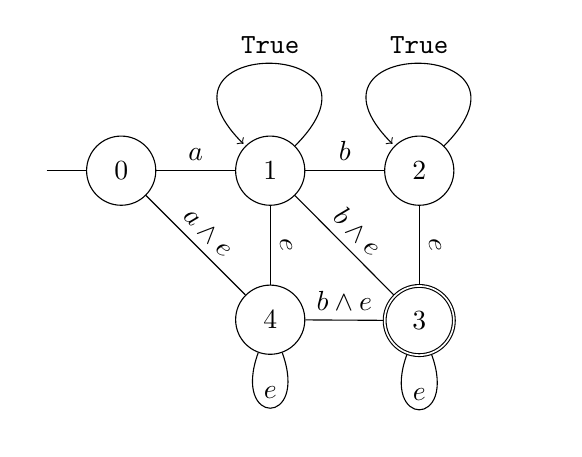
\begin{tikzpicture}	[node distance = 1cm]
		\node (init) {};
		\node [state, right=0.5cm of init](0) {0};
		\node [state, right=of 0] (1) {1};
		\node [state, right=of 1] (2) {2};
		\node [state, accepting, below=of 2] (3) {3};
		\node [state, below=of 1] (4) {4};
		
		\path [every node/.style={above, sloped}]
			(init) edge (0) 
			(0) edge node {$a$} (1)
			(0) edge node {$a \land e$} (4)
			(1) edge [loop] node [above] {\texttt{True}} (1)
			(1) edge node {$b$} (2)
			(1) edge node {$b \land e$} (3)
			(1) edge node {$e$} (4)
			(2) edge [loop] node {\texttt{True}} (2)
			(2) edge node {$e$} (3)
			(3) edge [min distance=10mm, in=250, out=290] node {$e$} (3)
			(4) edge node {$b \land e$} (3)
			(4) edge [min distance=10mm, in=250, out=290] node {$e$} (4)
		;
		\end{tikzpicture}
	\end{subfigure}
	\begin{subfigure}[t]{0.4\textwidth}
		\caption{MFSM}
		\centering
		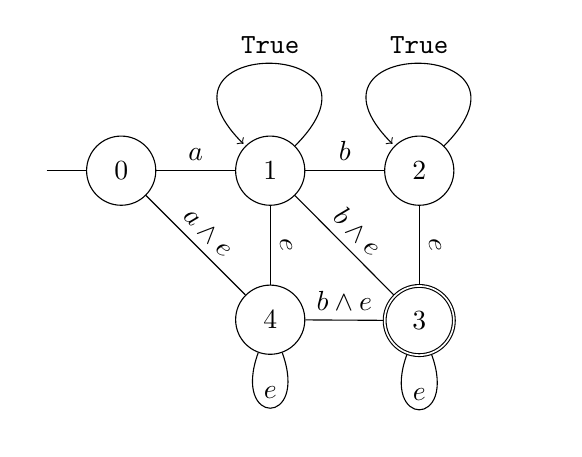
\begin{tikzpicture}	[node distance = 1cm]
		\node (init) {};
		\node [state, right=0.5cm of init](0) {0};
		\node [state, right=of 0] (1) {1};
		\node [state, right=of 1] (2) {2};
		\node [state, accepting, below=of 2] (3) {3};
		\node [state, below=of 1] (4) {4};
		
		\path [every node/.style={above, sloped}]
			(init) edge (0) 
			(0) edge node {$a$} (1)
			(0) edge node {$a \land e$} (4)
			(1) edge [loop] node [above] {\texttt{True}} (1)
			(1) edge node {$b$} (2)
			(1) edge node {$b \land e$} (3)
			(1) edge node {$e$} (4)
			(2) edge [loop] node {\texttt{True}} (2)
			(2) edge node {$e$} (3)
			(3) edge [min distance=10mm, in=250, out=290] node {$e$} (3)
			(4) edge node {$b \land e$} (3)
			(4) edge [min distance=10mm, in=250, out=290] node {$e$} (4)
		;
		\end{tikzpicture}
	\end{subfigure}

	\begin{subfigure}[t]{0.45\textwidth}
		\caption{Collapsing}
		\centering
		\begin{tikzpicture}	[node distance = 1cm]
		\node (init) {};
		\node [state, right=0.5cm of init](0) {0};
		\node [state, right=of 0] (1) {1};
		\node [state, accepting, below=of 2] (3) {3};
		\node [state, below=of 1] (4) {4};
		
		\path [every node/.style={above, sloped}]
			(init) edge (0) 
			(0) edge node {$a$} (1)
			(0) edge node {$a \land e$} (4)
			(1) edge node {$b \lor (b \land e)$} (3)
			(1) edge node {$e$} (4)
			(3) edge [min distance=10mm, in=250, out=290] node {$e$} (3)
			(4) edge node {$b \land e$} (3)
			(4) edge [min distance=10mm, in=250, out=290] node {$e$} (4)
		;
		\end{tikzpicture}
	\end{subfigure}
	\begin{subfigure}[t]{.35\textwidth}
		\caption{BTT-FSM}
		$[s_0] \rightsquigarrow a ? (e ? s_1 s_4 : s_1) : \emptyset$

		$s_1 \rightsquigarrow b ? (e?s_3 s_4 : s_3) : (e ? s_4 : \emptyset)$

		$s_3 \rightsquigarrow e ? s_3 : \emptyset$

		$s_4 \rightsquigarrow e ? (b?s_3 s_4 : s_3) : \emptyset$
	\end{subfigure}
\end{figure}

\textcolor{red}{
	The answer to $a\land\circ(\F b)\land \F(\G(e))$ after collapsing is wrong.
	Node 1 is also a total SCC and goes to accepting state, so it can be collapsed.
}

\end{enumerate}

\bibliographystyle{plain}
\bibliography{ref}

\end{document}